\begin{question}
\noindent A space agency uses a grid to model the movement of a rover exploring a rectangular survey site on the surface of Mars. Shape $M$ is translated to shape $N$, as shown on the grid below.

\begin{center}
\scalebox{0.75}{%
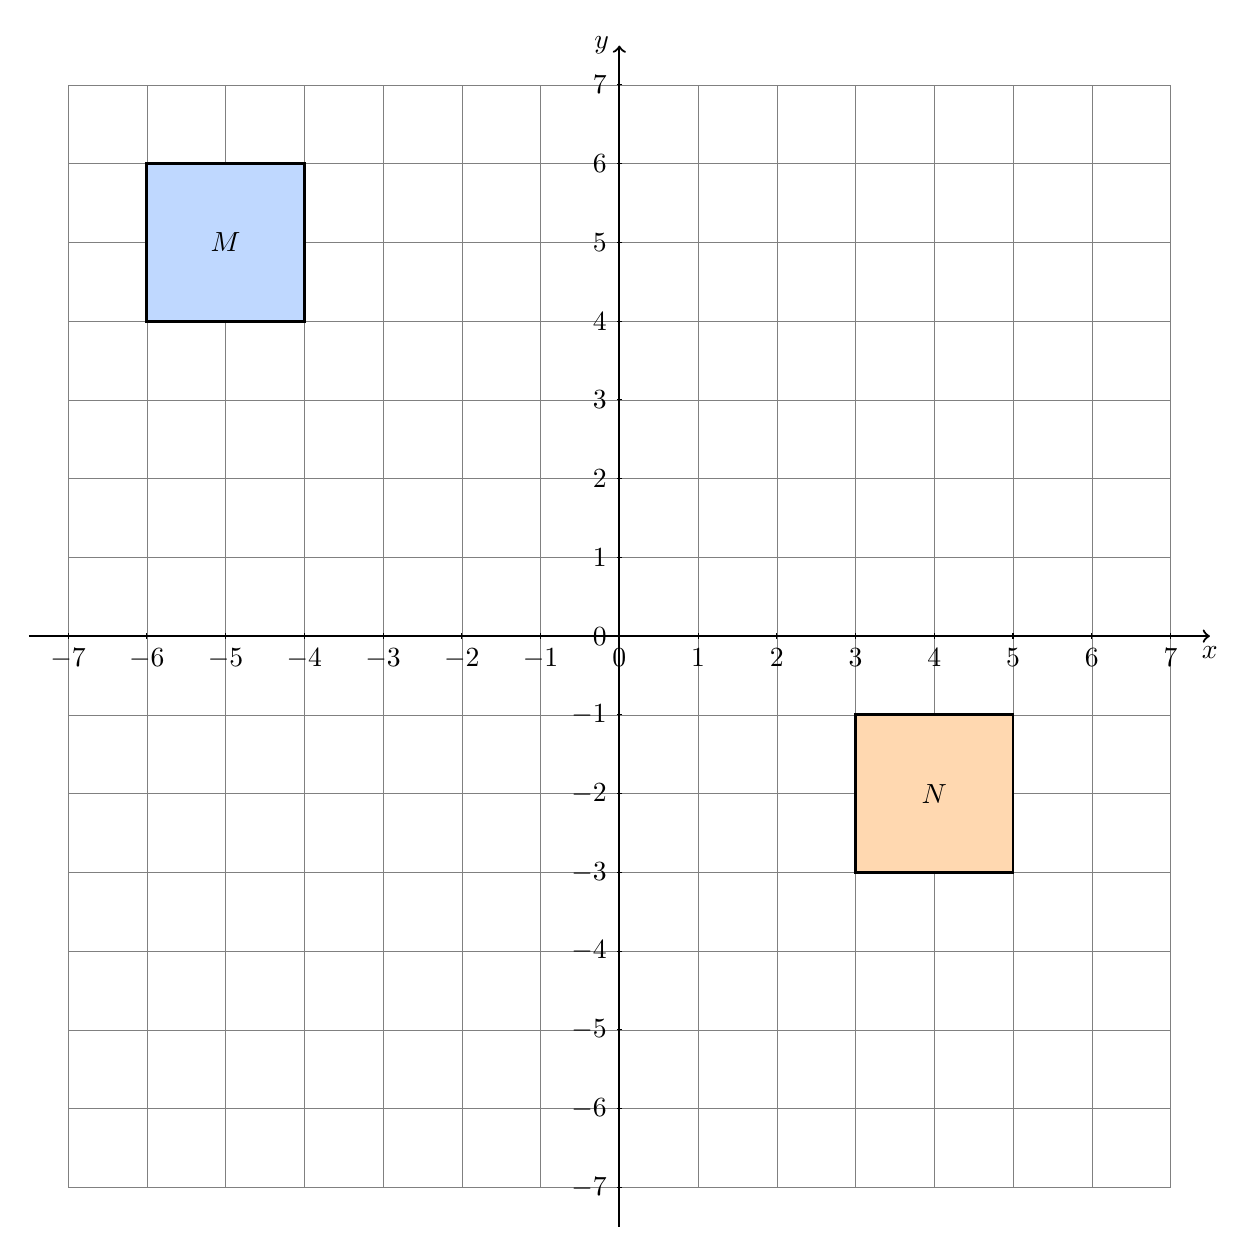
\begin{tikzpicture}
    \def\axisLimit{7}
    \definecolor{borderColour}{HTML}{000000}
    \definecolor{fillColourM}{HTML}{BFD8FF}
    \definecolor{fillColourN}{HTML}{FFD8B0}

    % Draw grid
    \draw[step=1cm,gray,very thin] (-\axisLimit,-\axisLimit) grid (\axisLimit,\axisLimit);

    % Draw axes
    \draw[thick,->] (-\axisLimit-0.5,0) -- (\axisLimit+0.5,0) node[anchor=north] {$x$};
    \draw[thick,->] (0,-\axisLimit-0.5) -- (0,\axisLimit+0.5) node[anchor=east] {$y$};

    % Label x-axis and y-axis
    \foreach \x in {-\axisLimit,...,\axisLimit}
        \draw (\x cm,1pt) -- (\x cm,-1pt) node[anchor=north] {$\x$};
    \foreach \y in {-\axisLimit,...,\axisLimit}
        \draw (1pt,\y cm) -- (-1pt,\y cm) node[anchor=east] {$\y$};

    % Shape M: vertices (-6,4), (-6,6), (-4,6), (-4,4)
    \coordinate (A) at (-6,4);
    \coordinate (B) at (-6,6);
    \coordinate (C) at (-4,6);
    \coordinate (D) at (-4,4);
    \filldraw[fill=fillColourM, draw=borderColour, line width=1pt] (A) -- (B) -- (C) -- (D) -- cycle;
    \node at (-5,5) {$M$};

    % Shape N: translate M by (9,-7): vertices (3,-3),(3,-1),(5,-1),(5,-3)
    \coordinate (Ap) at (3,-3);
    \coordinate (Bp) at (3,-1);
    \coordinate (Cp) at (5,-1);
    \coordinate (Dp) at (5,-3);
    \filldraw[fill=fillColourN, draw=borderColour, line width=1pt] (Ap) -- (Bp) -- (Cp) -- (Dp) -- cycle;
    \node at (4,-2) {$N$};

\end{tikzpicture}%
}
\end{center}

\noindent Describe fully the single transformation that maps shape $M$ onto shape $N$.

\vspace{4cm}

\begin{flushright}
    \answerplain{2}
\end{flushright}
\end{question}
